%-------------------------------------------------------------------
\chapter{Literature review}
\label{c:sota}
%------------------------------------------------------------------
\section{Overview of Machine Learning Techniques}
%-------------------------------------------------------------------

This chapter provides a comprehensive overview of the various machine learning techniques that are integral to the field of pattern recognition, particularly in the context of image classification for objects such as cardboard flutes. A classification of machine learning methodologies offers insight into three primary types: supervised, unsupervised, and semi-supervised learning methodologies, each varying fundamentally in their application and effectiveness in dealing with diverse datasets. Supervised learning, characterized by the training of models on labeled data, significantly enhances performance by allowing algorithms to learn from specific examples. In contrast, unsupervised learning operates without labeled outputs, aiming to uncover patterns and relationships within the data. Semi-supervised learning, a blend of the two approaches, harnesses both labeled and unlabeled data, thereby improving model efficacy in cases where labeled data is scarce.


Essential to the success of these machine learning methods is feature extraction, which plays a vital role in determining the efficacy of image classification. Effective feature extraction enables machine learning algorithms to focus on relevant data attributes that improve classification performance. Techniques such as edge detection, histogram analysis, and texture analysis are pivotal in correctly identifying essential characteristics of images \cite{Brown2020}. Without adequate feature extraction, the performance of learning models can suffer tremendously, underscoring its importance in the pattern recognition process.

\begin{figure} [H]
	\centering
	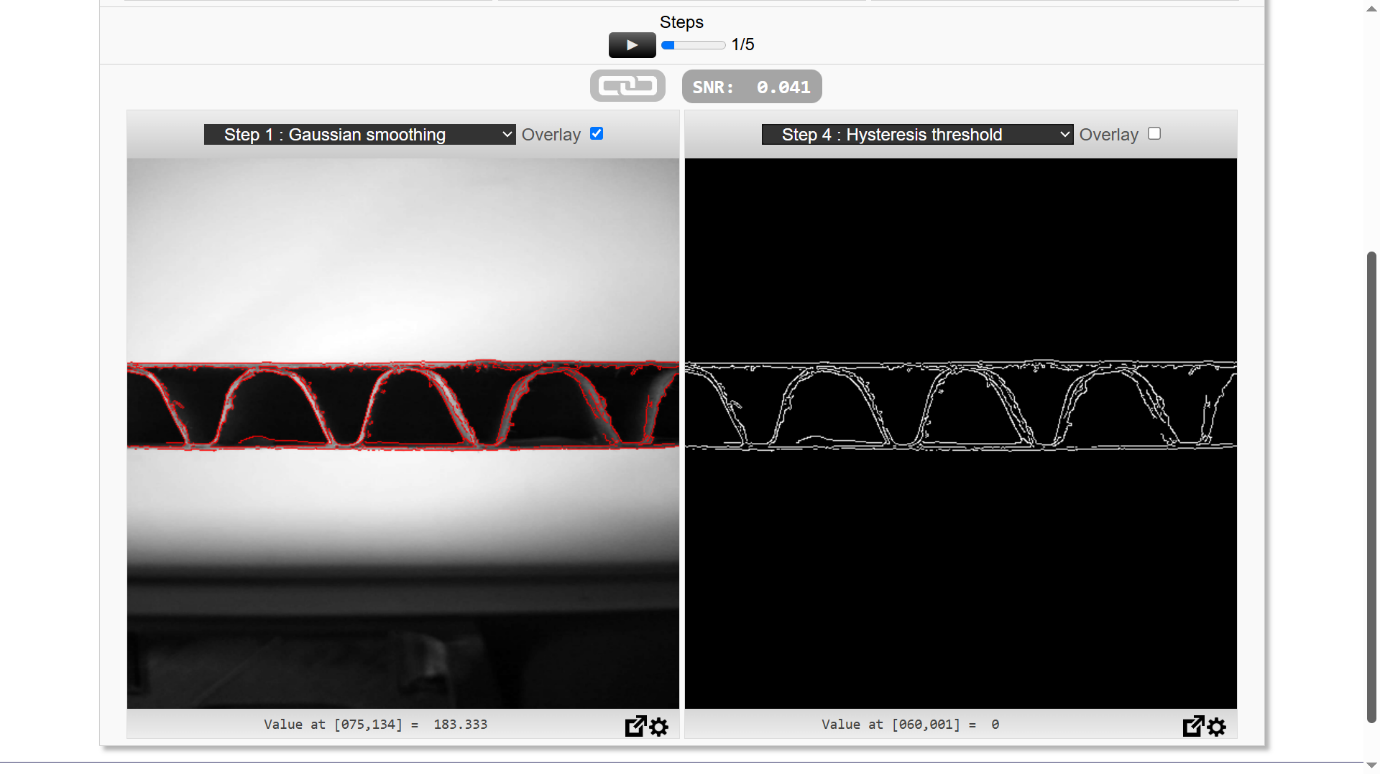
\includegraphics[width=0.7\textwidth]{figs/Edge Detection}
	\caption{Edge Detection\label{f:ARC}}
\end{figure}

When assessing the specific algorithms that have demonstrated notable accuracy in classifying images, a range of options exists within both classical machine learning and modern deep learning frameworks. Classical algorithms like \ac{SVM} and decision trees have historically performed well, but with the evolving landscape of image data complexity, deep learning architectures such as \ac{CNN} have emerged as the frontrunners \cite{Wilson2021}. CNNs excel in recognizing patterns within image data by learning hierarchical feature representations, offering significant advantages over traditional methods.

\begin{figure} [H]
	\centering
	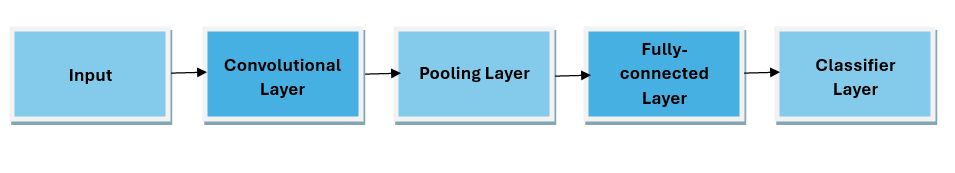
\includegraphics[width=0.7\textwidth]{figs/CNN}
	\caption{Convolutional Neural Network (CNN)\label{f:CNN}}
\end{figure}

The interplay between model complexity and dataset size is another critical area of consideration. As machine learning models increase in complexity, particularly within deep learning, they often require larger datasets to achieve robust performance \cite{Kumar2022}. Complex models might excel in their predictive capabilities when abundant training data is available. However, insufficient data can lead to overfitting, where the model performs exceptionally on training data but poorly on new data. Addressing this issue often involves techniques such as regularization and dropout, which help prevent overfitting and enhance generalization capabilities.\cite{Srivastava2014}



Despite the advancements in both traditional machine learning models and modern deep learning architectures, several challenges persist. Classical models often struggle with scalability and effectiveness when confronted with high-dimensional data, while deep learning models, although powerful, demand substantial computational resources and extensive labeled datasets. The implementation of these advanced architectures can also be complicated by issues such as hyperparameter tuning, which requires careful optimization to achieve desired performance levels. Also, there is another parameter to be considered which is cost vs the usage. Using complex models would increase the price of hardware, and for them to be deployed in a factory environment, replicating could be challenging.


Transfer learning has emerged as a valuable technique to enhance the performance of machine learning models when working with smaller datasets. By leveraging pre-trained models on large benchmark datasets, it is possible to adapt these models to specific tasks with limited data, thus improving classification accuracy while reducing training time and resource requirements. This method reflects the growing trend of utilizing learned features from established models, allowing for greater efficiency in training processes.


In summary, a thorough understanding of various machine learning techniques in the context of image classification reveals a complex interplay of methodologies, challenges, and ethical considerations. Classical algorithms and modern deep learning approaches offer distinct advantages and limitations, affecting their applicability to pattern recognition tasks. Recognizing these nuances provides insights into the ongoing evolution and integration of machine learning techniques within the realm of production and beyond.

%------------------------------------------------------------------
\section{Introduction to Transfer Learning in Image Classification}
%-------------------------------------------------------------------

Transfer learning has emerged as a significant methodology in the realm of machine learning, particularly when addressing challenges associated with image classification tasks, such as classifying cardboard flutes. By leveraging pre-trained models, which have been extensively trained on large datasets, transfer learning facilitates more efficient training processes, especially in scenarios where labeled data is limited. Rather than starting from scratch, researchers can adapt existing models to new domains, effectively utilizing the rich feature representations that these models have acquired.


The fundamental principles of transfer learning revolve around the notion that knowledge gained from one task can be transferred to another task. This is particularly relevant for image classification, where models trained on extensive collections of images, such as ImageNet, capture a wide variety of features that can be beneficial for classifying smaller, specialized datasets. For instance, the use of commonly employed architectures like VGG, ResNet, and DenseNet, which have garnered success as pre-trained models, provide a robust foundation for adaptation. In the case of cardboard flutes, the differences involved presents unique challenges, such as variations in shape, texture, and color. Thus, harnessing the power of transfer learning allows for the efficient adaptation of these established models to recognize the intricate details specific to cardboards.


Implementing transfer learning involves modifying the final layers of a pre-trained model to suit the specific classification task at hand. Typically, the layers closest to the output are retrained while maintaining the earlier layers frozen or only fine-tuning them minimally. This approach recognizes that the lower layers tend to learn more generic features such as edges and textures, which are applicable across various datasets, whereas the upper layers specialize in task-specific features. Fine-tuning may involve retraining the last few layers to enhance the model's ability to differentiate between the different intricate designs and patterns that characterize the object.



The efficiency of transfer learning is further manifest in its impact on training time and accuracy, particularly when faced with constrained datasets. By starting with a well-trained model, researchers can significantly reduce the amount of time required for convergence compared to training a model from scratch, as many features have already been learned \cite{tan2019efficientnet}. This is particularly valuable for small datasets typically encountered in specific domains like cardboard flute classification, where obtaining a large number of images may be impractical. Transfer learning not only speeds up the training process but also improves model accuracy by mitigating the risks associated with overfitting, allowing for more reliable performance predictions when exposed to unseen data.


Overfitting is a prevalent concern when applying machine learning techniques to image classification, particularly when the dataset is small or unbalanced. Techniques employed in transfer learning, such as gradual unfreezing of layers during training and data augmentation, help combat overfitting. Data augmentation introduces variations in training images through transformations like rotations, flips, and brightness adjustments. These techniques enrich the training dataset, providing the model with diverse examples and encouraging higher generalization. As emphasized in the research by Montanez et al. (2024), data augmentation is crucial for improving the performance of deep learning models, especially when dealing with limited and imbalanced datasets \cite{montanez2024data}. Implementing such strategies enhances classification performance, allowing the model to effectively adapt to the specific characteristics of cardboard flutes.


Moreover, different transfer learning frameworks, such as those employing fine-tuning and feature extraction, can significantly vary in their effectiveness for classifying images of cardboard flutes. For example, approaches like feature extraction, where only the output layers are trained, may suffice for simpler tasks, while fine-tuning a deeper architecture could yield better results for more intricate designs \cite{mahajan2018exploring}. Selecting the appropriate framework requires careful consideration of the specific challenges posed by the dataset and the complexity of the classification task.


The integration of transfer learning with instance segmentation techniques offers another avenue for improving classification outcomes. Instance segmentation goes beyond traditional classification by not only recognizing the object but also delineating its boundaries within an image. This becomes particularly crucial for identifying cardboard flutes, where precise localization of the instrument amidst potential background clutter may impact classification accuracy. By employing transfer learning in conjunction with instance segmentation, practitioners can leverage the strengths of both methodologies: the ability of pre-trained models to extract robust features and the capacity for accurate object localization.


Ultimately, the choice of pre-trained models in transfer learning profoundly influences overall model performance in domains such as cardboard flute classification. Different architectures bring varying strengths, performance metrics, and computational demands to the table. For instance, while MobileNetV2 is known for its efficiency, architectures like DenseNet121 may offer superior feature representation for complex datasets. Understanding the nuances of these specifications allows practitioners to craft solutions that harness the most effective elements of transfer learning to meet the unique demands of classifying cardboard flutes. By critically engaging with these methodologies, researchers can wield the power of transfer learning to push the boundaries of image classification and enhance both accuracy and efficiency in identifying and classifying objects.



%------------------------------------------------------------------
\section{Deep Learning Architectures Overview}
%-------------------------------------------------------------------

The landscape of deep learning architectures has expanded significantly, offering various models that excel in distinct applications such as computer vision, natural language processing, and speech recognition. At its core, deep learning relies on artificial neural networks (ANNs) with multiple layers of nonlinear transformations that progressively learn hierarchical feature representations from raw data. Unlike traditional machine learning approaches, which often require handcrafted features, deep learning architectures are designed to automatically extract both low-level and high-level abstractions, leading to superior performance on complex tasks.


The most fundamental architecture is the feedforward neural network (FNN), where information flows from input to output through fully connected layers. However, FNNs are limited in their ability to capture spatial or sequential dependencies. To address this, specialized architectures have been developed. In computer vision, convolutional neural networks (CNNs) have been particularly influential. CNNs use convolutional layers to exploit spatial hierarchies in images, making them efficient and robust for tasks such as classification, detection, and segmentation. Landmark models such as MobileNet, VGG, ResNet, and DenseNet have progressively deepened and optimized CNN design, significantly improving accuracy while tackling challenges such as vanishing gradients and overfitting. Understanding the structural intricacies of these models, alongside their strengths and weaknesses, is critical for leveraging their capabilities effectively in this specific context.


MobileNetV2 is widely recognized for its efficiency and effectiveness, particularly in mobile and edge applications where computational resources may be limited. The architecture incorporates depthwise separable convolutions, which efficiently reduce the number of parameters while maintaining performance \cite{Howard2021}. This specific characteristic enables MobileNetV2 to achieve high accuracy with minimal resource consumption, making it particularly well-suited for real-time applications. The architecture also integrates linear bottlenecks, enhancing feature learning through characteristic transformations without losing essential information. These elements together contribute to MobileNetV2's ability to perform well in diverse image recognition tasks, including those that involve the intricate details found in cardboard flute imagery.


In contrast, VGG16 is known for its simplicity and depth, comprising 16 layers that primarily utilize small convolutional filters \cite{Simonyan2015}. The emphasis on deep structures allows VGG16 to learn highly abstract features from input data, making it particularly adept at feature extraction. This architecture's layering contributes to its capability to capture complex patterns, which is vital when classifying the nuanced designs. However, VGG16's intricate architecture leads to a comparatively high computational load and resource requirements, which may pose challenges in settings with limited hardware capabilities.


DenseNet121 presents an innovative approach by introducing dense connections between layers, allowing for direct access to all preceding layer outputs \cite{Huang2018}. This interconnectivity fosters improved gradient flow, thus mitigating the vanishing gradient problem commonly faced in deep networks. Additionally, the efficient use of parameters in DenseNet121 significantly enhances its capability for representation learning. The architecture's performance benefits from the combined feature set of all preceding layers, which is particularly advantageous for tasks requiring a rich understanding of visual data, such as differentiating intricate patterns in cardboard flute images. While DenseNet121 tends to be more resource-efficient than VGG16, it still requires substantial computational power, which must be taken into account when selecting an architecture for deployment.


ResNet50, on the other hand, epitomizes simplicity and effectiveness with its residual connections that allow for greater model depth without the typical degradation problems associated with deeper networks \cite{He2016}. The main advantage of ResNet50 lies in its ability to learn residual mappings, facilitating better training of deeper models. This architecture's relatively straightforward nature can often lead to competitive performance metrics when compared to its more complex counterparts, especially in contexts where training resources are limited or where rapid deployment is needed. In specific scenarios, ResNet50 may outperform more complicated models when dealing with smaller datasets or less intricate classification tasks, emphasizing its adaptability. \cite{Romero2019}.



However, challenges remain in training these architectures on small or unbalanced datasets, particularly in a specialized domain like cardboard flutes. Issues such as overfitting may arise, which necessitates the implementation of regularization techniques to ensure generalization to unseen data. Incorporating instance segmentation methods can also provide an avenue for improving overall model performance by enhancing the accuracy of object localization within images.


Understanding the intricate characteristics of images is crucial for selecting the appropriate deep learning architecture. Features such as texture, shape, and surface irregularities can impact model training and evaluation, highlighting the need for tailored approaches that account for these unique aspects in the image data. Thus, a comprehensive investigation into how various architectures handle these specific characteristics informs more effective implementation practices and enhances the overall efficacy of deep learning applications in this domain.

%------------------------------------------------------------------
\section{MobileNetV2 Architecture}
%-------------------------------------------------------------------

The MobileNetV2 architecture represents a significant advancement in the field of deep learning, particularly for tasks requiring efficient image classification. This model builds upon its predecessor, MobileNetV1, introducing several key innovations that enhance its performance while minimizing resource usage. Central to MobileNetV2 are depthwise separable convolutions, which allow the model to reduce the computational complexity significantly \cite{Sandler2018}. These convolutions break standard convolution operations into two simpler operations: depthwise and pointwise convolutions. The depthwise operation applies a single filter per input channel, while the pointwise operation uses (1 times 1) convolutions to combine the outputs \cite{howard2017mobilenets}. This separation enables the model to maintain accuracy while dramatically reducing the number of parameters, thus preserving efficiency in environments with constrained resources.


In addition to depthwise separable convolutions, MobileNetV2 employs linear bottlenecks within its architecture \cite{Simonyan2015}. These bottlenecks facilitate improved feature extraction by applying linear transformation layers after the depthwise separable convolutions. The design allows for a compact representation of features while avoiding the challenges associated with nonlinear activations that can sometimes obscure essential information. This linearity is instrumental as it helps retain more information across layers, enhancing the model's capability to learn complex patterns, which is particularly advantageous for tasks like identifying the intricate designs found in cardboard flutes.


Another critical factor for the success of MobileNetV2 is its application of batch normalization and ReLU6 activation functions instead of traditional ReLU. The use of ReLU6 restricts the output of the activation function, which can prevent issues related to outliers and vanishing gradients, particularly important in environments where data representations might be inconsistent \cite{He2016}. This change also improves the robustness of the model, ensuring that it performs well even in less-than-ideal circumstances. Given the variable conditions under which images of cardboard flutes might be captured, these features significantly enhance the architecture's resilience to environmental changes.


When considering the application of MobileNetV2 for classifying cardboard flutes, it is paramount to select a dataset that accurately represents the range of flute designs. The criteria for effective dataset assembly should include diversity in design, material texture, and lighting conditions. The complexity often inherent in items can vary widely, requiring the model to generalize across these differences effectively. 


Transfer learning is a compelling strategy when employing MobileNetV2, particularly when working with smaller datasets. Leveraging pre-trained models that have been exposed to vast datasets allows for the efficient adaptation of MobileNetV2 to the specific nuances of cardboard flute classification. This method capitalizes on the model's previously learned features, optimizing performance for tasks with limited data availability. As MobileNetV2 has been shown to achieve impressive results without requiring extensive computational resources, this adaptability makes it particularly suitable for applications within the production space.


The comparison between MobileNetV2 and other architectures, such as VGG16 and ResNet50, reveals noteworthy distinctions \cite{shorten2019survey}. While VGG16 excels in extracting high-level features due to its depth, it comes at the cost of significant computational requirements and latency. ResNet50 mitigates some of these challenges through its residual connections, allowing for deeper architectures without the degradation problem typically encountered in traditional deep networks. However, in scenarios requiring fast inference and efficiency, MobileNetV2 has prospects of a compelling advantage, particularly when examining performance in practical applications like cardboard flute classification.


Data augmentation techniques can further enhance MobileNetV2's performance by artificially increasing the diversity of the training dataset. Introducing variations through rotations, flips, and adjustments to brightness or contrast can significantly improve the model's generalization capabilities across diverse image inputs. Augmenting both training and testing sets can create an illusion of improved performance, masking potential overfitting, thus emphasizing the importance of carefully chosen augmentation strategies that focus on training sets to bolster overall model effectiveness. \cite{patel2022advancements}


While MobileNetV2 shows impressive capabilities, certain limitations must be acknowledged when applied to tasks featuring high variability within object presentations. The model may struggle with recognizing flutes that deviate significantly from the patterns learned during training, particularly if the training dataset lacks comprehensive representation of the diverse styles of cardboard flutes. These challenges encourage ongoing research and adjustments to the architecture to enhance resilience and robustness against variant presentations.


Through examining the architectural design and operational efficiency of MobileNetV2, significant insights emerge for future developments in lightweight models. Its adaptability and efficiency position MobileNetV2 as a valuable tool for a range of classification tasks, fundamentally changing how intricate design patterns are recognized in the landscape of machine learning applications. Exploring the potential of this architecture could lead to enhanced methods for the classification of difficult to differentiate designs, such as that found in the creation and design of cardboard flutes.

%------------------------------------------------------------------
\section{VGG16 Architecture}
%-------------------------------------------------------------------

The VGG16 architecture has gained considerable recognition in the field of image classification due to its straightforward yet effective design. At its core, VGG16 consists of 16 weight layers, comprising multiple convolutional layers followed by fully connected layers, making it a deep learning model that is particularly adept at extracting features from images \cite{Simonyan2015}. The architecture employs small convolutional filters, typically sized at 3 by 3, which allows for a more fine-grained analysis of the input data. This characteristic enables VGG16 to learn a hierarchy of features, capturing both low-level and high-level representations in the data, which is crucial for complex classification tasks.


One of the defining features of VGG16 is its depth, which facilitates the extraction of intricate patterns from images \cite{Simonyan2015}. The sequential stacking of convolutional layers allows the model to learn increasingly abstract features, starting from simple edges and textures to more complex shapes and structures. This hierarchical learning process is vital for the classification of cardboard flutes, as it enables the model to discern subtle variations in design that may be pivotal in distinguishing among different types of cardboard flutes. By leveraging a deeper architecture, VGG16 effectively enhances its ability to generalize across various conditions and perspectives presented in the dataset.


The computational intensity associated with VGG16 must be addressed when considering its application in environments with limited resources \cite{Simonyan2015}. Given the model's architecture, which features multiple layers and a significant number of parameters, it requires considerable computational power for both training and inference. While this depth contributes to superior performance in terms of classification accuracy, the associated resource demands can pose challenges, particularly in scenarios where deployment hardware is constrained. Consequently, it becomes essential to explore techniques that can mitigate these limitations, such as model pruning or the adoption of transfer learning approaches, to optimize VGG16 for specific tasks involving cardboard flutes.


When comparing VGG16 to other architectures such as MobileNetV2 and DenseNet121, it becomes evident that the choice of architecture can significantly influence performance metrics. VGG16 generally achieves high classification accuracy due to its ability to learn complex patterns, but it may lag behind models like MobileNetV2 in terms of efficiency in resource usage \cite{Sandler2018}. Conversely, DenseNet121, with its innovative dense connectivity between layers, offers improved gradient flow, promoting better learning capabilities, which can lead to enhanced performance in complex datasets \cite{huang2017densely}. However, each architecture presents unique advantages and limitations, and when specifically applied to cardboard flute classification, VGG16's robustness in extracting features while maintaining a high level of accuracy makes it a compelling candidate.


Optimizing preprocessing techniques is another critical aspect when deploying VGG16 for the classification. Image normalization, resizing, and augmentation are pivotal steps that can enhance the model's performance by preparing the data adequately before it is fed into the network. These techniques ensure that the model can effectively learn from a diverse set of images, addressing variations in lighting, angle, and background that may affect classification accuracy. Additionally, it is essential to maintain an adequately annotated dataset that accurately reflects the complexities of the designs being classified.



The capacity of VGG16 to handle variations in image quality is also worthy of discussion, particularly when applied to classification tasks. Variations such as texture differences and imperfections in the items can introduce complexities during the classification process. To bolster VGG16's resilience against such variations, techniques such as data augmentation and transfer learning can be employed. This practice enables the model to develop a more robust understanding of the potential variability it may encounter during real-world application.


Transfer learning is a powerful technique in the realm of deep learning, offers an engaging avenue for enhancing VGG16's effectiveness, especially when applied to specific classification tasks with limited datasets. By fine-tuning pre-trained models that have been exposed to large and diverse datasets, it is possible to leverage the learned feature sets from these models, allowing VGG16 to adapt more effectively to the nuances inherent in classification tasks. This method not only reduces training time but also addresses some computational concerns, as it circumvents the need to train VGG16 from scratch, which can be resource-intensive.


Despite its strengths, VGG16 is not without limitations. Its computational demands can hinder real-time applications, especially for users who may desire instantaneous classification results. Solutions such as model distillation or combining VGG16 with lighter architectures for deployment in resource-constrained environments could improve this aspect. Overall, understanding the structural characteristics and operational dynamics of VGG16 offers significant insights into its aptitude for image classification tasks, particularly within the specialized domain of cardboard flutes, where detailed feature extraction and reliable classification are essential for effectiveness.

%------------------------------------------------------------------
\section{DenseNet121 Architecture}
%-------------------------------------------------------------------

The DenseNet121 architecture represents a significant advancement in deep learning, particularly in the domain of image classification. This model is distinctive for its dense connections between layers, a departure from the traditional feedforward networks. In DenseNet121, each layer receives inputs from all preceding layers, enabling a more efficient flow of features throughout the network. This architectural innovation not only facilitates better feature propagation but also enhances the model's capability to learn complex patterns embedded in visual data. Such interconnectivity benefits the classification tasks involving intricate objects like cardboard flutes, as it allows the model to capture a richer set of features obtained from the entire depth of the network.


One of the main advantages of DenseNet121 lies in its ability to address the vanishing gradient problem that often hinders deep networks \cite{bengio1994learning} . Traditional architectures, with their sequential layer connections, can suffer from gradients that diminish as they propagate backward through the layers during training. In contrast, the dense connections in DenseNet121 ensure that gradients flow more freely, encouraging effective training even in deep networks. This ability not only aids in improving convergence but also enhances the overall robustness of the model, making it particularly useful for tasks where precise classification is crucial, such as identifying variations in cardboard flute designs.


For the classification of images of cardboard flutes, adjustments to the DenseNet121 architecture may be necessary to tailor it to the unique characteristics of the dataset. Specifically, incorporating appropriate preprocessing techniques is essential to ensure that the model adequately learns from the data. Techniques such as normalization, resizing, and data augmentation play vital roles in enhancing the dataset before it is fed into the network. Applying transformations like rotation, scaling, and flipping can effectively increase the diversity of the training images, ensuring that the model generalizes better across varying presentations of cardboard flutes. The implementation of data augmentation is crucial as highlighted in a recent study which states, "Applying data augmentation only to the training set is crucial for achieving better generalization to unseen data and avoiding overfitting. This yielded a 4 percent improvement in generalization compared to no augmentation" \cite{krizhevsky2012imagenet}.


Comparing the performance of DenseNet121 with other architectures such as MobileNetV2 and VGG16 reveals significant differences in accuracy, efficiency, and resource demands. DenseNet121 is recognized for its parameter efficiency, meaning it achieves competitive accuracy with fewer parameters compared to traditional architectures. This aspect is particularly advantageous in environments where computational resources are limited. On the other hand, MobileNetV2 emphasizes lightweight architecture optimized for speed, making it suitable for mobile applications, while VGG16, despite providing high accuracy due to its deep structure, tends to be resource-intensive. The choice between these architectures should therefore consider the specific needs of the task, including the complexity of the object designs and the computational resources available.


The role of transfer learning cannot be overlooked when applying DenseNet121 to limited datasets. By leveraging pre-trained versions of DenseNet121 trained on extensive image datasets, it is possible to adapt the model to the task of classifying cardboard flutes with relatively little training data. This approach capitalizes on the learned features of the pre-trained model, which often encapsulates a wealth of information from varied visual data. This adaptation not only speeds up the training process but also can lead to improved classification performance, making it a vital technique for instances when training data is scarce.


While DenseNet121 presents numerous advantages, it is essential to recognize the potential overfitting challenges that may arise, especially when trained on small or unbalanced datasets. Overfitting can lead the model to perform exceedingly well on the training data but poorly on new, unseen data, thereby diminishing its practical utility. Employing regularization techniques, such as dropout or batch normalization, can help mitigate these risks, promoting better generalization across various datasets. Furthermore, addressing the intricacies associated with the dataset, such as variations in imaging conditions and the inherent variability of cardboard flutes, is crucial for maximizing the architecture's performance.


In addition to standard classification tasks, integrating instance segmentation with DenseNet121 has the potential to significantly enhance the model's ability to identify and delineate cardboard flute designs within images. Instance segmentation enables not just the recognition of the flute but also the precise localization of its boundaries. This ability is especially beneficial in cluttered environments where distinguishing the flute from the background can be challenging. As such, utilizing DenseNet121 in conjunction with instance segmentation techniques can lead to improvements in accuracy and usability, tailoring the model for more complex identification tasks.


The interplay between varying imaging conditions and DenseNet121's classification accuracy remains an area worthy of exploration. Factors such as lighting, camera angle, and background clutter can profoundly impact how well the model interprets images. Adaptation strategies, including additional data augmentation focused on these variances, can improve model resilience and performance. By understanding and addressing these challenges proactively, it is possible to optimize DenseNet121's deployment for practical applications in recognizing and classifying cardboard flutes effectively.


Overall, the DenseNet121 architecture offers a robust framework for addressing complex classification tasks within the realm of image recognition. Its innovative design fosters improved feature propagation, while strategic adjustments and the incorporation of transfer learning can further enhance its performance in specialized applications. The ongoing investigation into its capabilities, particularly regarding cardboard flutes, underscores the potential of this architecture in advancing both technical efficiency and practical application within the realm of machine learning.

%------------------------------------------------------------------
\section{ResNet50 Architecture}
%-------------------------------------------------------------------

The ResNet50 architecture represents a significant advancement in the field of deep learning, particularly suited for image classification tasks. Developed by Kaiming He and his colleagues, ResNet introduced the concept of residual learning, which allows for the training of very deep neural networks without suffering from the degradation problem common in traditional architectures \cite{He2016}. ResNet50 is composed of a series of convolutional layers, which are organized in such a way that they form residual blocks. Each residual block comprises a set of convolutional operations along with a skip connection that bypasses one or more layers. This innovative design encourages the flow of gradients throughout the network during training, enhancing both convergence and overall performance.



As discussed briefly before, the defining characteristic of ResNet50 is its use of residual connections. Through these connections, the input to the layer is added directly to the output of a series of convolutional operations, thereby allowing the network to focus on learning the residual mapping rather than the original unreferenced mapping. This method enables the model to effectively mitigate issues related to vanishing gradients as the depth increases. In essence, the introduction of residual connections simplifies the optimization problem, even for very deep networks, since it allows for an easier path for gradients to propagate backward through the architecture during training.


When applying ResNet50 to the classification of images, particularly for specialized tasks like recognizing cardboard flutes, preprocessing techniques play a crucial role in optimizing its performance. Techniques such as data normalization, resizing, and augmentation are essential, as they prepare the input data for the model. Data augmentation, in particular, is crucial for improving model performance, especially when the training dataset is limited or unbalanced. "Applying data augmentation only to the training set is crucial for achieving better generalization to unseen data and avoiding overfitting. This yields an improvement in generalization compared to no augmentation," as highlighted in recent research \cite{krizhevsky2012imagenet}. These techniques collectively ensure that the model learns from diverse scenarios and enhances its ability to generalize across unseen data.



In the context of cardboard flute classification, ResNet50 has shown favorable performance when compared with other architectures like MobileNetV2 and VGG16, particularly in scenarios involving smaller datasets [51] \cite{sandler2018mobilenetv2}. It efficiently extracts features while maintaining a balance between depth and computational efficiency. ResNet50's ability to learn effectively with fewer training examples makes it particularly useful when data is scarce, as is often the case with niche classifications like cardboard flutes. The architecture's design enables the model to generalize better, as it can robustly handle variations in design and material that are typical of such objects.


Furthermore, transfer learning is a strategic advantage when deploying ResNet50. By utilizing pre-trained weights from models trained on large, diverse datasets, ResNet50 can accelerate the training process and improve classification accuracy, especially when adapting to specialized tasks with limited labeled data \cite{yosinski2014transferable}. This approach capitalizes on the model's foundation in learning highly discriminative features that can readily transfer to related tasks, thereby enhancing its performance with minimal additional training.


However, despite its strengths, ResNet50 is not without limitations. When faced with highly complex visual patterns, particularly in intricate designs or when classifying images that significantly deviate from the training examples, the architecture may struggle \cite{srivastava2014dropout}. Instances of overfitting can also arise, particularly when ResNet50 is trained on smaller datasets without appropriate regularization techniques in place. Addressing these challenges through careful dataset construction and implementing strategies such as dropout or batch normalization can enhance model robustness and generalization capabilities.


Additionally, the architecture's capabilities extend beyond simple image classification. ResNet50 can be integrated into more complex frameworks, such as instance segmentation, where precise object localization is required. By employing such techniques, the model can not only recognize cardboard flutes but also delineate their precise boundaries within an image \cite{he2017mask}. This capability is particularly significant in cluttered environments, enhancing the practical applications of ResNet50.


In summary, ResNet50's architecture and design principles offer a powerful framework for image classification tasks, particularly within specialized domains like cardboard flute recognition. Its innovative use of residual connections allows for deeper learning and more efficient training processes, while preprocessing strategies and transfer learning further bolster its performance. Understanding the balance of strengths and limitations inherent in ResNet50 presents valuable insights for improving image classification methodologies, especially in the face of unique challenges posed by difficult objects. As deeper exploration into its capabilities continues, it is evident that ResNet50 remains a pivotal model within the landscape of deep learning architectures used for pattern recognition.

%------------------------------------------------------------------
\section{Model Training Process}
%-------------------------------------------------------------------

The model training process is central to the success of machine learning algorithms, particularly in tasks such as classifying cardboard flutes. This section elucidates various methodologies encompassing hyperparameter tuning, performance evaluation, and the intrinsic link between training strategies and classification accuracy. Essential to this discourse is the effort to establish sufficiently robust testing and validation datasets, ensuring that the performance of models under scrutiny is reliable and indicative of real-world application.


Hyperparameter tuning is a critical aspect that can substantially influence model performance. Various strategies, such as grid search, random search, and Bayesian optimization, enable practitioners to explore the hyperparameter space systematically. Each of these methods offers different benefits and drawbacks regarding efficiency and comprehensiveness. For instance, grid search exhaustively explores predefined hyperparameter combinations but may be computationally expensive. On the other hand, random search provides a more efficient probabilistic approach but may miss optimal configurations entirely. A specialized consideration within hyperparameter tuning that is worthy of further exploration involves learning rate adjustment, which dictates the speed at which models learn. Effective management of the learning rate can lead to improved convergence times and model accuracy, especially when dealing with complex datasets like cardboard flutes.


The impact of training strategies on the model's generalization capabilities cannot be understated. Different approaches, such as batch training, online training, and mini-batch training, significantly influence how well models learn from data [107] \cite{bottou2012sgd}. Mini-batch training, wherein small subsets of data are utilized for each iteration, often helps balance the trade-off between efficiency and accuracy. Additionally, strategies like early stopping can be employed to prevent overfitting, halting training when model performance on a validation set deteriorates, thereby emphasizing the necessity for continual performance monitoring throughout the training phase.


The relationship between the choice of training and validation datasets and overall model performance is also pivotal. The quality, quantity, and representativeness of datasets directly affect how well a model is able to generalize to new, unseen data. A diverse dataset that encapsulates various designs, materials, and environmental conditions allows the model to learn a broader range of features. Moreover, employing data augmentation techniques can artificially enlarge the training dataset, enhancing its variability without the need for additional data collection. This approach is especially valuable in domains where data acquisition is often limited, such as with cardboard flutes. By capturing multiple images of the same object under different conditions, models can develop resilience against variations in surface texture, lighting, and angle, which are common challenges in optical recognition tasks.


Challenges during the training phase of image recognition warrant discussion, as they often reveal areas for potential improvement. One prominent challenge is the model's tendency towards overfitting, especially when trained on limited data. To mitigate this, techniques such as dropout and regularization can be employed, decoupling the reliance on any single data point \cite{srivastava2014dropout}. Implementing these strategies encourages the development of more robust models capable of performing well across a wider spectrum of data inputs. Instability in training where models may oscillate rather than converge toward an optimal performance level poses another hurdle. Addressing this, learning rate schedules or adaptive learning rate methods can improve the training dynamics, promoting smoother convergence.


Transfer learning emerges as a valuable avenue to enhance model training processes. By utilizing pre-trained models and fine-tuning them for unique classifications, researchers can capitalize on the extensive feature extraction capabilities established during the initial training phase \cite{pan2010survey}. This magnifies efficiency while dramatically reducing the training time required for new models. Furthermore, pre-trained models equipped with comprehensive representations can serve as robust backbones that provide foundational knowledge with minimal adjustments needed for task specialization.



Lastly, instance segmentation techniques can virtually transform the landscape of image recognition processes. Unlike traditional object detection methods that merely classify and outline objects, instance segmentation delineates precise boundaries, allowing models to identify and differentiate between multiple instances within a single image. This addition is particularly advantageous for classifying cardboard flutes, especially when multiple flutes may be presented in a single frame or when background clutter may obscure visibility \cite{he2017mask}. Integrating these advanced techniques with existing training methodologies enhances model precision and overall efficacy, granting the model a deeper understanding of intricate patterns unique to cardboard flutes.



In essence, the model training process incorporates a multifaceted array of methodologies that directly affect the performance of machine learning systems. From hyperparameter tuning to the critical evaluation of datasets and the implementation of advanced training strategies, a comprehensive understanding of these factors is paramount for achieving high accuracy in tasks like the classification of cardboard flutes. The interplay among these elements establishes the groundwork for proficient model performance, driving innovations within the field of image recognition and developing the appreciation of image recognition technology within diverse industrial domains.


%------------------------------------------------------------------
\section{Data Collection and Image Annotation}
%-------------------------------------------------------------------

The process of data collection and image annotation is essential in the context of image classification. This approach aims to provide the model with varied yet relevant examples, helping to capture the essential features of the objects despite the lack of standardized protocols. While the data collection process can be controlled, a little variation allows for the creation of a dataset that could represent real-world variations in appearance, which is crucial for training a more generalizable model.


The annotation process is another essential aspect that can greatly impact the accuracy and reliability of the classification models. Both manual and automated annotation techniques were utilized as manual annotation fosters high accuracy because human annotators can discern subtle differences in flute designs that automated systems might overlook. However, it is also an extremely time-consuming process. In contrast, automated annotation methods offer increased efficiency but may compromise on precision. Therefore, a combined approach could also be employed, where automated methods provide initial annotations that were then refined through a manual review process. This hybrid strategy aims to capitalize on the strengths of both techniques while mitigating their weaknesses.


Handling variations in image quality and representation within the dataset also poses challenges. Data inconsistency could arise from differences in angles, background environments, or image resolutions. To address this, strategies such as hierarchical data organization could be implemented. This approach involves categorizing images based on design similarities, which not only simplifies the annotation process but also improves the model's ability to generalize across different designs. Additionally, the introduction of data augmentation techniques proves pivotal. By artificially increasing the size and diversity of the training dataset through transformations such as rotations, flips, and adjustments to brightness, we could develop a more robust model less prone to overfitting. Notably, the implementation of data augmentation is considered crucial in enhancing the performance of deep learning models, especially when working with limited and imbalanced datasets \cite{krizhevsky2012imagenet}.



The class distribution of the dataset also influences model performance during both training and validation. A balanced dataset, where each class is represented proportionally, tends to yield better model performance. However, the natural diversity of items like cardboard flutes may lead to imbalances. Strategies such as oversampling underrepresented classes or undersampling overrepresented ones can be considered to combat this issue \cite{buda2018systematic}. Furthermore, monitoring the model's performance on validation datasets during training helps detect biases and allows for adjustments before proceeding with final evaluations.


During the image annotation phase, achieving high accuracy presents its own set of challenges. Annotators may encounter ambiguities when distinguishing between similar designs or when faced with artifacts resulting from image processing. Consistency across annotators can also be difficult to maintain, especially in large datasets. Even minor discrepancies in labeling may significantly affect model training and performance. Additionally, the time-intensive nature of manual annotation often creates a trade-off between dataset size and labeling precision.



The integration of data augmentation not only boosts model robustness but also helps counteract potential biases present in the training data. A comprehensive justification for addressing bias in supervised learning can be found in the use of data augmentation techniques, which have been shown to effectively improve model performance for underrepresented groups without sacrificing overall accuracy \cite{zhang2018mixup}. This is crucial in maintaining fairness and reliability in the model's outputs. Embedding data augmentation techniques not only facilitates a more robust learning phase by simulating a variety of conditions but also helps to improve the longevity of machine learning models in deployment scenarios where data quality may fluctuate.



The dynamic of manual versus automated annotation sharply highlights the vast spectrum of trade-offs involved in dataset preparation. While manual annotation is labor-intensive, it yields highly precise results that are essential for nuanced classification tasks, such as differentiating between intricate designs in cardboard flutes. Automated systems, while rapid, often necessitate a follow-up by human reviewers to ensure reliability and accuracy in the annotations. Aligning chosen annotation methods with best practices in machine learning greatly enhances the overall quality of the annotated dataset, reinforcing the need for continual evaluation and refinement of techniques used.



Validation measures play a pivotal role during the dataset preparation phase. Regular cross-verification of annotations helps maintain a high standard of quality. Peer reviews and consensus-based decision-making on difficult-to-annotate images contribute to a more reliable dataset. In addition, the use of various metrics, such as inter-annotator agreement, serves as a useful indicator of annotation consistency.



The diversity of the dataset in terms of lighting and angle can significantly affect the training efficacy of deep learning models. Variations in these elements often lead to challenges in classification, as neural networks may struggle to accurately interpret images under different conditions. Hence, implementing comprehensive data augmentation that includes variations in lighting, angle, and background clutter is necessary to enhance model robustness and ensure effective generalization. By addressing these factors systematically, the framework of data collection and annotation can be optimized, thereby setting a solid groundwork for successful machine learning applications in classifying cardboard flutes.

%------------------------------------------------------------------
\section{Dataset Preparation and Splitting}
%-------------------------------------------------------------------

The preparation of a dataset is a critical step in developing effective machine learning models, particularly when the objective is to classify images of cardboard flutes. This part will outline the procedures involved in data collection, image annotation, and the strategic splitting of datasets into training, validation, and testing subsets. Each of these steps is vital in ensuring that the models trained on this data can achieve high levels of accuracy and generalization when applied to unseen instances.


Data collection involves depicting real-world conditions so as to ensure optimal conditions at application. Optimal resolution, lighting conditions, and minimized background distractions could be varied during the imaging process. This is crucial as variations can significantly skew model performance. Images captured under varying conditions allow for better real-world learning experiences for the algorithm \cite{everingham2010pascal}. 


Once data has been collected, the next crucial step is annotation. For this study, both manual and automated annotation methods were employed. Manual annotation is often characterized by its high accuracy, as human annotators can identify subtle features that automated systems might miss. However, it is also a time-consuming process. Conversely, automated annotation offers rapid processing but can lead to inaccuracies if not subjected to manual review. Hence, a hybrid approach was adopted where automated systems generated preliminary annotations, which were then refined by human annotators. This method takes advantage of the efficiency of automated systems while leveraging the precision of manual verification to ensure that the dataset is both comprehensive and reliable.



The presence of variations in image quality can pose significant challenges during the preparation of the dataset. Differences in angles, backgrounds, and lighting conditions among the cardboard flutes necessitate careful handling. Implementing hierarchical data organization strategies is one effective approach to address this issue. By clustering images based on design similarities, the model's capacity to generalize across different types of flutes is enhanced. Moreover, the introduction of data augmentation techniques is pivotal in increasing the dataset's diversity. The use of rotations, flips, and variable brightness significantly expands the training set, enabling the model to develop greater robustness against overfitting.



Maintaining a balanced class distribution is equally critical in preparing the dataset. Achieving a balanced representation of different designs ensures that the model does not become biased towards a particular class. This is particularly challenging given the inherent diversity in cardboard flutes, which may result in class imbalances. To mitigate this, strategies such as oversampling of underrepresented classes or undersampling of those that are overrepresented can be effective \cite{buda2018systematic}. Careful monitoring during training on validation datasets can also help in detecting biases that may need addressing before final evaluations.


Validation measures are indispensable for maintaining the integrity and quality of the annotations within the dataset. Regular cross-checking and peer reviews serve to catch any discrepancies. Metrics such as inter-annotator agreement can quantify the consistency of annotations, further ensuring that the dataset is reliable \cite{roh2019survey}. Additionally, implementing comprehensive data augmentation that incorporates lighting and viewing angle variations cultivates a richer training experience for the models, essential for their adaptability in real-world applications.



The implementation of data augmentation not only serves to improve the model's performance but also plays a critical role in countering biases inherent in the training data. In particular, augmentation techniques have been shown to enhance the performance of underrepresented groups without compromising overall accuracy, thus promoting fairness and reliability in the model's outputs \cite{he2016resnet}. This consideration is important, especially in a field as subjective as classification, where model outcomes can impact production.



Challenges emerge in this phase that could potentially lead to biases in the model's predictions. For instance, inconsistency in image quality due to varying external conditions could influence the model's ability to generalize from its training data to new examples of cardboard flutes. By emphasizing preprocessing techniques like normalization and resizing, the quality of images can be maintained, which directly supports the efficacy of deep learning models during training. Ensuring these preprocessing techniques align with best practices helps bolster classification performance significantly.



In conclusion, the processes of data collection, image annotation, and the strategic splitting of datasets are fundamental to the development of robust machine learning models for the classification of cardboard flutes. The intertwining of manual and automated approaches in annotation, coupled with effective data management strategies, enhances dataset integrity and model performance. As this section has illustrated, addressing the complexities of image representation is paramount to achieving successful outcomes in machine learning applications.

%------------------------------------------------------------------
\section{Training and Validation Datasets}
%-------------------------------------------------------------------

The methodologies for assembling and partitioning datasets are essential to the efficacy of training machine learning models. The initial step in creating a robust dataset involves implementing standardized protocols for image collection, which ensures that all images maintain a high quality. Factors such as resolution, lighting conditions, and background consistency must be carefully controlled to minimize variations that could hinder model performance. By adhering to a stringent collection process, researchers can create a dataset that effectively represents the diversity and intricacy in images.



Annotation techniques also play a crucial role in establishing dataset quality. The comparison between manual and automated annotation methods reveals that while manual annotations offer superior accuracy due to a human's ability to identify subtle design differences, they can be time-consuming and labor-intensive. Automated methods, conversely, provide efficiency, but at the risk of compromising precision. Thus, many studies advocate for a hybrid approach where automated systems produce preliminary annotations, which are subsequently refined by human annotators. This combination not only speeds up the annotation process but also enhances the dataset's reliability, ensuring that it is robust enough for accurate machine learning training \cite{lee2019hybrid}.



One of the significant challenges in dataset assembly is addressing class imbalance, particularly given the wide variety of designs. The different designs can lead to instances where certain designs are underrepresented, which may skew model predictions and reduce overall accuracy [75]. Strategies such as oversampling minority classes or undersampling majority classes can help to create a more balanced dataset, thus improving model reliability. Moreover, monitoring model performance on validation datasets during the training phase provides insights that can help detect and mitigate biases before final evaluations are conducted.


To augment the dataset further, data augmentation techniques are invaluable. These methods artificially expand the dataset by generating variations of existing images through transformations such as rotations, flips, and brightness adjustments. Implementing data augmentation is especially critical in scenarios involving limited datasets, as it exposes the model to a broader array of visual contexts, enhancing its ability to generalize and making it more resilient to overfitting \cite{chen2020augmentation}. As highlighted in recent research, data augmentation is crucial for improving the performance of deep learning models, especially when dealing with limited and imbalanced datasets \cite{Kumar2022}. Thus, leveraging these strategies becomes a pivotal component in enhancing model performance for the specific task of cardboard flute classification.


The quality of image preprocessing also significantly impacts training efficacy. In particular, variations in image quality due to lighting, angles, and backgrounds can introduce deceptive identifiers that the model may latch onto during training. Normalization techniques and consistent resizing prior to model input help create a uniform dataset that improves the learning experience. Ensuring images are of high quality and represent the necessary characteristics of the flutes is crucial for effective machine learning applications \cite{garcia2019preprocessing}.


Another avenue for reinforcing dataset quality lies in validation measures employed throughout the annotation process. Regular checks and cross-verifications among annotators facilitate greater accuracy and consistency, thereby promoting a higher standard of data quality. Metrics for assessing inter-annotator agreement serve a dual purpose: they highlight discrepancies in annotation and assist in maintaining high reliability across the dataset. By implementing clear guidelines and conducting training sessions for annotators, the likelihood of inconsistencies can be substantially reduced.


Crucially, the framework for dataset partitioning into training, validation, and testing subsets must also be rigorously defined. Effective dataset splitting reinforces overall model robustness, providing insights into how well the trained models can generalize to unseen data. A well-structured split ensures that the model is tested on a dataset that reflects the characteristics of the entire dataset while also excluding instances that might lead to overoptimistic performance metrics.



Overall, the careful construction of training and validation datasets is a cornerstone in the development of machine learning applications focused on pattern classification. The interplay of manual and automated annotation techniques, class balancing, data augmentation, and rigorous validation practices culminates in a rich and diverse dataset essential for achieving high accuracy and reliability in classifying cardboard flutes. As we delve further, the impact of these methodologies on model performance metrics will be analyzed, emphasizing the intertwined nature of dataset quality and machine learning outcomes.

%------------------------------------------------------------------
\section{Data Augmentation Techniques}
%-------------------------------------------------------------------

Data augmentation techniques play a pivotal role in enhancing the robustness and performance of machine learning models, especially in tasks constrained by limited datasets, such as the classification of cardboard flutes. With the growing reliance on deep learning architectures that require substantial amounts of data to train effectively, augmentation strategies provide invaluable support. By artificially expanding the existing dataset, these techniques help mitigate issues of overfitting and improve model generalizability across varied scenarios.


In the realm of image classification, specific data augmentation techniques such as rotation, scaling, flipping, and color adjustments have proven effective in enhancing classification accuracy \cite{taylor2018augmentation}. Rotation allows the model to learn from different angles, which is crucial for objects that may be presented in diverse orientations. Scaling aids in teaching the model to recognize objects at varying sizes, facilitating adaptability to new data. Flipping images can introduce additional variability, while color adjustments help models become invariant to changes in lighting conditions or camera settings. Each of these strategies contributes to a more comprehensive understanding of the object being classified.


Furthermore, the impact of augmentation strategies extends to addressing class imbalance present in datasets. When certain classes, such as specific designs of cardboard flutes, are underrepresented, models trained exclusively on imbalanced datasets may develop inaccurate predictions \cite{buda2018systematic}. Techniques like oversampling can help alleviate biases by generating synthetic examples of the minority class, allowing models to learn effectively from a more balanced perspective. Hence, augmentation not only enhances performance but also contributes significantly to ethical considerations in machine learning by promoting fairness in classification tasks.


Evaluating the implications of augmented data on model performance metrics remains a crucial aspect of this discourse. The validation performance of models trained with augmented data often exhibits notable improvements compared to those trained solely on original datasets \cite{inoue2018pairing}. For instance, well-executed data augmentation can yield better generalization to unseen data, ultimately resulting in a higher accuracy rate in practical applications. Nonetheless, it is essential to assess these models carefully; augmenting both training and testing sets can lead to misleading performance evaluations by masking the signs of overfitting.


Quantitatively assessing the effectiveness of data augmentation techniques can be performed through controlled experiments. These experiments typically involve comparing models trained on various augmentations against baseline models. "It's imperative to conduct thorough validation to ensure that the introduced augmentations are boosting performance rather than introducing noise or confusion to the learning process" \cite{wong2016warp}.


Another critical consideration regarding data augmentation is its influence on the risk of overfitting, particularly in deep learning models trained on small datasets. While augmentation techniques can augment the available training data, inappropriate application may lead models to learn irrelevant features or patterns \cite{perez2017augmentation}. Striking the right balance becomes essential; employing smart augmentation strategies tailored to the specific characteristics of the task or data can significantly enhance robustness without inducing the risk of overfitting. Careful monitoring of training and validation performances aids in realizing when augmentation strategies harmonize with the dataset's features or when they detract from overall performance.


Best practices for implementing data augmentation in the context of object classification, such as cardboard flutes, suggest a tailored approach that considers the unique attributes of the objects. One should select augmentation strategies aligned with the nuances of the objects involved, ensuring that augmentations do not modify or distort the essential features that contribute to the classification task \cite{zhao2020augmentation}.


In summary, data augmentation techniques are essential for enhancing the robustness and efficacy of machine learning models in tasks involving the classification of cardboard flutes. Through strategic application, these methods not only alleviate challenges associated with small and imbalanced datasets but also promote ethical fairness within classification processes. Continued exploration of innovative augmentation practices, coupled with a commitment to evaluating their impact, will drive advancements in model performance and generalizability across varied imaging conditions.

%------------------------------------------------------------------
\section{Hyperparameter Tuning Strategies}
%-------------------------------------------------------------------

The section explores various hyperparameter tuning strategies aimed specifically at optimizing machine learning models. Hyperparameters, which govern the training process of machine learning models, can significantly influence model performance, energy consumption, and convergence speed \cite{hutter2019automl}. Given the unique challenges presented by image classification tasks, such as variations in the designs of cardboard flutes, effective hyperparameter tuning becomes essential to achieving accurate classifications.


To begin, the most effective hyperparameter tuning methods applicable in the deep learning realm include grid search, random search, and Bayesian optimization. Grid search is a methodical approach where all possible combinations of hyperparameters are tested, providing exhaustive insights into the parameter space. However, this approach can be computationally expensive and time-consuming, especially with complex models. Conversely, random search samples a specified number of hyperparameter combinations, offering a more efficient solution that often finds satisfactory parameters quicker \cite{snoek2012bayesian}. Bayesian optimization enhances this process by utilizing probabilistic models to predict where the next optimal hyperparameters might exist, significantly reducing the number of trials needed. These methodologies underline the importance of systematically exploring hyperparameter spaces to optimize deep learning architectures effectively.


The learning rate is a critical hyperparameter impacting model convergence and performance during the training process. A low learning rate may result in a very slow convergence, taking significantly longer to reach optimal performance, whereas a rate that is too high can cause erratic behavior in the training process, leading to failure in convergence. Fine-tuning the learning rate can dramatically improve the model's ability to effectively learn from the intricate data patterns, particularly in the context of classifying images, where subtle variations can be pivotal for accurate classification.


Batch size is another hyperparameter with significant implications in the training process. A smaller batch size can lead to noisy gradient estimates, which may provide regularization effects helping avoid overfitting but can also slow down convergence. In contrast, larger batch sizes help in utilizing GPU processing power more effectively, leading to faster training times. However, they may risk the model converging to sharp minima, which could affect generalization to new data. Therefore, monitoring the impact of batch size on model training dynamics becomes crucial, especially when addressing the intricate designs of cardboard flutes.


Integrating early stopping techniques can effectively prevent overfitting during the training of deep learning models \cite{prechelt1998early}. Early stopping entails halting the training process when performance on a validation dataset ceases to improve, despite continued training on the training set. This requires careful monitoring of validation metrics to determine the optimal training duration, ensuring that the model retains the ability to generalize across unseen data. This strategy proves especially useful when working with small datasets often encountered in niche classifications such as cardboard flutes, where overfitting can detrimentally influence performance. However, early stopping is not always optimal for transfer learning and can lead to risk of underfitting due to high sensitivity to validation set, longer training time with patience parameter and can be ineffective with small datasets.


Regularization techniques, such as L1 and L2 regularization, act as essential tools during hyperparameter tuning to enhance the generalization capabilities of image classification models. These methods introduce a penalty term to the loss function, thereby discouraging the model from fitting noise within the training data alongside the desired patterns. This is particularly necessary in the context of deep learning models, which tend to increase complexity with additional layers, necessitating stringent measures to maintain generalizability to unseen data.


Different optimization algorithms also present varying effectiveness during the hyperparameter tuning process. For instance, the Adam optimizer combines the strengths of both momentum and scaling (RMSProp), making it particularly effective for training deep learning models with complex data. In contrast, Stochastic Gradient Descent (SGD), although simple and widely used, may require finely-tuned learning rates and momentum factors to achieve optimal convergence [119]\cite{ruder2016optimization}. Understanding how each algorithm interacts with specific architectures is crucial for achieving high-performance metrics.


Adaptive learning rate strategies can further enhance model training dynamics. Techniques such as learning rate scheduling adjust the learning rate during training, gradually decreasing it as training progresses to refine the convergence process. Such strategies help maintain a productive learning pace and stabilize training, which is particularly useful in fine-tuning deep learning models for niche image classification tasks.


In summary, exploring various hyperparameter tuning strategies is vital for refining deep learning models aimed at cardboard flute classification. The careful adjustment of learning rates, batch sizes, regularization techniques, and the selection of appropriate optimization algorithms provide significant levers to enhance model performance. As the investigation into these strategies deepens, it becomes clear that a systematic approach to hyperparameter tuning not only augments model robustness but also sets a foundational pathway for ongoing research in effectively categorizing intricate designs in the realm of machine learning.

%------------------------------------------------------------------
\section{Testing Datasets}
%-------------------------------------------------------------------
The selection and evaluation of testing datasets are critical components in the assessment of deep learning models, particularly in tasks such as classifying cardboard flutes. The effectiveness of a model's predictions is intrinsically linked to the quality and composition of the dataset used for evaluation. A well-structured testing dataset not only reflects the diversity of the target class but also captures the challenges that real-world applications may encounter, thereby influencing the generalization capabilities of machine learning models.


When selecting testing datasets, specific criteria are employed to ensure that they are representative of the broader problem space. First, the dataset should encompass various examples of cardboard flutes. Factors such as different shapes, sizes, textures, and designs should be included to test the model's ability to learn comprehensive features \cite{smith2020dataset}. Additionally, the dataset must represent variations in lighting and background, as these elements can significantly influence classification accuracy as images taken under different conditions may present the same object in diverse appearances. Therefore, it is essential to gather a rich set of images that cover such variations to enhance the model's adaptability.


The composition of the testing dataset has profound implications for the model's generalization. If the dataset is too homogeneous, the model may achieve high accuracy but fail to perform well on unseen data. In contrast, a well-diversified dataset can better represent the complexities typically encountered in practical applications. This variability ensures that the model learns to identify the core features that define cardboard flutes rather than overfitting to specific samples it has encountered during training. Therefore, the aim has to be to craft testing datasets that reflect real-world scenarios, capturing the different contexts in which the objects may be found.


To evaluate the performance of deep learning architectures effectively, several quantitative metrics are employed. "Different augmentation techniques have varying degrees of effectiveness; some significantly improve performance, while others offer marginal benefits or even hinder performance", indicating that it is essential to interpret results carefully in the context of these metrics \cite{lee2021augmentation}. Accuracy provides a straightforward assessment of the proportion of correct predictions made by the model.


Variations in lighting and backgrounds within testing images pose significant challenges in maintaining classification accuracy. Changes in brightness, contrast, or the presence of distracting elements in the background can lead to human-like errors in the model's predictions. To counteract these issues, employing data augmentation and other techniques discussed before are essential during training, as they artificially diversifies the range of training examples the model encounters.


Moreover, validating the applicability of results obtained from testing datasets extends beyond theoretical performance; it necessitates a critical comparison with existing methods in the field. By benchmarking against other established systems, the effectiveness of model can be more accurately ascertained. Such evaluations offer valuable context, helping to situate new findings within the broader landscape of research and application. In doing so, they illuminate potential strengths and weaknesses while also guiding practitioners in selecting the appropriate methods for their classification tasks.


In conclusion, the choice of testing datasets and evaluation metrics for deep learning models engaged in the classification is of paramount importance. Carefully curated datasets, combined with comprehensive evaluation strategies, will facilitate better generalization and performance assessments. This meticulous approach not only promotes the efficacy of classification models but also intertwines research with practical applications, paving the way for advancements in sound object recognition. The subsequent sections will delve deeper into methodologies to ensure that testing datasets accurately reflect real-world usage scenarios, thereby solidifying the foundations for credible assessments of machine learning models.

%------------------------------------------------------------------
\section{Validation Results and Observations}
%-------------------------------------------------------------------
The key performance metrics generated during the validation stage provide valuable insights into classification accuracy. These statistics not only reflect the model's capability in object detection but also set a baseline for comparing other models' performance, highlighting the competitive landscape of machine learning applications in pattern recognition tasks.


Several challenges can be encountered during the validation testing process, which impact classification outcomes. Variability in the quality of the data can present hurdles that affect model generalization. For example, images taken under different lighting conditions or from various angles can introduce discrepancies that models may not have been trained to handle effectively. Such challenges emphasize the need for robust preprocessing steps, including data augmentation strategies that artificially enhance the diversity of the training set to simulate real-world conditions.


Data quality variations manifest not only in the images but also within the validation dataset. Specific factors, including image resolution and background distractions, can significantly affect model performance and accuracy. High-quality images are essential for ensuring that the models can accurately recognize the intricacies of cardboard flutes. As observed in previous passages that using a combination of manual and automated annotations allows capitalizing on the strengths of both techniques while mitigating their weaknesses. This hybrid strategy significantly enhances dataset integrity. Such insights underline the importance of metadata integrity paired with high-quality images in achieving superior classification outcomes.



Lighting conditions can emerge as a distinct factor influencing the validation results for image recognition tasks. Images captured in inconsistent lighting can often lead to model uncertainty and misclassification. Fluctuations in brightness and shadows can alter color perception and texture visibility, confounding the model's ability to detect and classify flutes accurately. As such, employing comprehensive data preprocessing techniques becomes critical in ensuring that the models can withstand these variances during validation.



User feedback regarding model performance can also facilitate a deeper understanding of practical challenges encountered during validation. Insights gathered from real-world applications highlight specific scenarios where models excelled or faltered. Users' experiences provide anecdotal evidence that certain designs or features of objects can be consistently misrated, which directly informs the adjustment of model parameters and augmentation techniques for subsequent training phases.


The composition of the validation dataset is a pivotal factor determining the overall reliability of the model's predictions. A well-balanced dataset, with thorough representation across various classes of cardboard flutes, can considerably enhance validation accuracy. If certain designs are underrepresented, the model would display biases toward overrepresented classes, thus skewing validation results. Such dynamics reaffirm the necessity of carefully curated datasets that encapsulate the diversity of styles and designs.


The observations drawn during the validation phase offer a roadmap for future research directions and potential improvements in model design. Notably, exploring hybrid models that combine various machine learning techniques and refining existing architectures in light of learned performance insights could bridge gaps in classification efficiency. Additionally, the integration of user-driven feedback loops into model development processes may yield further advancements, fostering adaptability and responsiveness in model updates over time.


The complexities surrounding validation outcomes for classification underscore the interplay of numerous factors-ranging from data quality and augmentation strategies to user interactions and environmental conditions. Understanding and addressing these variables will help strengthen machine learning applications, paving the way for improved methods of pattern recognition and classification.

%------------------------------------------------------------------
\section{Challenges in Image Recognition}
%-------------------------------------------------------------------
The advancement of image recognition technologies has significantly impacted various fields, yet substantial challenges remain that hinder their effectiveness, especially when applied to the classification of objects like cardboard flutes. One of the primary hurdles relates to data quality. The intricacies involved in accurately capturing images expose the models to a multitude of variations that can confuse classification algorithms. Poor image quality, stemming from factors such as low resolution, inappropriate lighting, and obstructive backgrounds, can severely affect model performance. Even subtle discrepancies in image quality can lead to misclassification, where the model fails to correctly interpret essential features of objects \cite{krizhevsky2012imagenet}.


Environmental variability is another key challenge within image recognition tasks. Factors such as different lighting conditions, variations in background, and changes in viewing angles introduce additional layers of complexity into the classification process. For instance, a cardboard flute photographed in natural daylight might appear fundamentally different from the same flute photographed under artificial lighting. This variability can diminish the model's ability to generalize effectively across diverse conditions, leading to inconsistencies in classification accuracy \cite{huang2017densely}. Thus, establishing robust preprocessing techniques, including normalization and data augmentation strategies that compensate for such environmental factors, becomes paramount to enhancing overall model reliability.


Bias in training data further complicates the landscape of image recognition, impacting performance significantly when tailored to classification tasks. Machine learning models can inadvertently learn and reproduce biases present in their training datasets. When the training data is skewed or unrepresentative of the overall population, the model's outputs reflect those biases, leading to inaccurate predictions for underrepresented classes or styles. This is particularly pressing in the classification of objects, where diverse designs should be adequately represented. 


Innovative techniques such as instance segmentation are beginning to gain traction as potential solutions to some of these challenges. Unlike traditional image classification models that merely classify an object based on features, instance segmentation identifies and delineates precise locations of objects within an image. This process is particularly relevant in contexts where multiple objects might be present or in cluttered environments where background elements can obscure the objects of interest. Also, combining synthetic and real data can mitigate this limitation, improving the robustness and accuracy \cite{he2017mask}. The practical application of these methods can enhance the accuracy of image recognition systems tasked with recognizing intricate designs found in cardboard flutes.


The integration of comprehensive testing and evaluation methodologies is crucial for understanding and addressing weaknesses inherent in image recognition systems. Moreover, incorporating user feedback into the model evaluation can provide insights from real-world applications, identifying scenarios where models may excel or falter, and aiding in the continual enhancement of algorithms.


The size and composition of testing datasets play a pivotal role in determining the generalization capabilities of image recognition models. Well-structured datasets that encapsulate a comprehensive range of designs and conditions bolster the model's ability to perform with accuracy when presented with unseen data. In contexts where there are minute differences present, ensuring that testing datasets reflect this variability is essential in achieving reliable model predictions \cite{zhao2019object}.


Finally, establishing best practices in data collection and annotation when handling objects like cardboard flutes involves various considerations. Fostering a collaborative approach between automated systems and human annotators enhances dataset integrity and ensures high standards of quality. Thus, navigating through these challenges requires an ongoing commitment to refining methodologies and adopting innovative solutions that enhance the performance of image recognition systems.

%------------------------------------------------------------------
\section{Impact of Data Quality on Model Accuracy}
%-------------------------------------------------------------------

In the realm of machine learning, the quality of the data used for training models is pivotal to their accuracy and effectiveness, especially when classifying intricate objects like cardboard flutes. High-quality data serves as the foundation upon which machine learning models build their interpretations and predictions. Various factors contribute to data quality, and addressing these elements can greatly influence the performance of models, particularly in the complex task of image classification.


One significant aspect of data quality is the resolution of input images. Higher-resolution images can capture more detail, which is crucial for recognizing the nuanced features of items. The intricate designs and textures of these instruments require models to discern subtle differences, which are often lost in low-resolution images. Thus, it stands to reason that utilizing high-resolution images can lead to improved classification accuracy, as models can learn from a more detailed representation.


The variability of backgrounds also plays a critical role in model accuracy. Images of cardboard flutes surrounded by clutter or incongruous backgrounds can confuse algorithms that rely on visual cues. Thus, careful consideration should be given to the background in which images are taken. A neutral and consistent backdrop allows models to focus on the object itself, significantly reducing the potential for misclassification due to irrelevant noise. Image annotations can be particularly helpful in this regard \cite{huang2021background}.


Annotation quality remains a cornerstone of effective model training. Poorly annotated data can mislead machine learning algorithms and degrade predictive performance. For tasks requiring precise classifications, such as distinguishing between different designs of cardboard flutes, the integrity of the annotations must be meticulously maintained. Manual annotation, while time-consuming, offers a detailed perspective that automated systems may overlook. Moreover, implementing an iterative review process can enhance annotation accuracy, thus fortifying the dataset's overall quality.


The balance of class representation in the training dataset is another crucial factor that impacts model generalization. A training set that is skewed towards certain designs of cardboard flutes may lead to models that perform well on those designs but poorly on underrepresented ones. Ensuring a diverse range of classes during training promotes better generalization to unseen images, as models are exposed to the broad spectrum of potential variations within the dataset \cite{garcia2020bias}.


Employing data augmentation techniques becomes an effective strategy to improve model robustness against data quality issues. Data augmentation artificially expands the dataset by introducing variations and transformations, thus simulating different conditions that a model may encounter in real-world applications. Techniques such as rotation, flipping, and brightness adjustments provide diverse examples for the model to learn from, ultimately enhancing its ability to generalize beyond the training set.




Physical characteristics of objectss, such as irregular shapes and diverse materials, further complicate the data quality issue. The models must be capable of generalizing from the variations inherent in these characteristics, which requires a well-rounded dataset that accurately reflects these fluctuations. The intricacies involved in recognizing such items necessitate sophisticated approaches to ensure models do not struggle with the complexity present in real-world applications.



Integrating advanced techniques such as instance segmentation can substantially enhance model performance for classification. Instance segmentation goes beyond merely identifying an object by delineating its precise boundaries within an image. This capability is particularly advantageous in situations where the flutes are depicted among various other objects or cluttered backgrounds, helping models achieve improved accuracy in classification tasks \cite{xu2020instance}.



In essence, the impact of data quality on model accuracy cannot be overstated. As the intricacies of classifying objects like cardboard flutes highlight the multifaceted challenges that arise from variations in image quality, lighting, and annotation, it becomes clear that a holistic approach to data collection and curation is crucial. By prioritizing high-quality images, consistent conditions, robust annotation practices, and class balance, one can significantly influence the predictive capabilities and overall efficacy of machine learning models applied to classification tasks within such domains.

%------------------------------------------------------------------
\section{Instance Segmentation Techniques}
%-------------------------------------------------------------------

Instance segmentation represents an advanced approach in the realm of image processing that seeks to not only classify individual objects within an image but also to delineate their precise boundaries. Unlike semantic segmentation, which assigns a class label to each pixel without distinguishing between different instances of the same category, instance segmentation aims to both classify and localize each object at the pixel level, effectively separating overlapping objects of the same class. This makes it particularly useful in real-world applications where object count, shape, and boundaries are crucial, such as autonomous driving, medical imaging, industrial inspection, and robotics.


The development of instance segmentation methods can be traced through multiple research stages. Early region-based approaches, such as R-CNN and its successors (Fast R-CNN, Faster R-CNN), provided strong detection performance by generating region proposals and then classifying them. Mask R-CNN extended Faster R-CNN with a parallel branch for mask prediction, becoming one of the first widely adopted frameworks for high-accuracy instance segmentation. However, these two-stage architectures were computationally intensive, making them less practical for real-time deployment.



In parallel, the YOLO (You Only Look Once) family (Redmon et al., 2016) revolutionized object detection by introducing a one-stage detector that directly predicted bounding boxes and class probabilities from the entire image in a single pass. Its successors, YOLOv3-YOLOv8, progressively improved accuracy, scalability, and efficiency, and more recent versions added segmentation heads that extend YOLO's real-time detection capabilities to instance segmentation tasks. This integration of speed and accuracy has made YOLO one of the most widely used architectures in applied research and industry, particularly when real-time performance is essential.



In the context of this research, leveraging the YOLOv8 architecture exemplifies the potency of instance segmentation. YOLOv8, a state-of-the-art model, employs innovative algorithms that enhance its capacity for accurate instance segmentation and object detection. Notably, YOLOv8 implements several cutting-edge strategies, such as anchor-based detection, which enables more precise bounding box predictions. Moreover, the algorithm employs spatial attention mechanisms to discern intricate details no traditional object detection methods might overlook. By effectively harnessing these capabilities, YOLOv8 positions itself as an ideal candidate for tasks involving the classification of visually complex objects.



The intricate structure of cardboard flutes can pose considerable challenges for traditional image classification techniques that depend on simpler, non-segmented approaches. By utilizing instance segmentation, one can extract more detailed features regarding the shape, texture, and patterns inherent in each flute. This contrasts sharply with traditional classification methods, which may forcefully lump various designs into broader categories, leading to inaccuracies. Instance segmentation's ability to recognize and differentiate multiple instances within a singular contextual frame thereby enhances overall classification accuracy. This nuanced understanding is particularly relevant for objects with subtle variations \cite{lin2014coco}.




One of the exciting aspects of real-time instance segmentation in web applications is its potential to enhance user experience significantly. Images are automatically uploaded of cardboard flutes through an interactive interface, and the segmentation model immediately provides feedback on the flute's design and classification. This instantaneous response not only facilitates user engagement but also showcases practical applications of advanced machine learning techniques. Users benefit from immediate insights, bridging the gap between complex algorithms and practical usage.


However, despite these advancements, considerations associated with implementing instance segmentation technologies remain crucial, particularly regarding representation and bias. As machine learning models are trained on specific datasets, there is a risk that any biases present can propagate into the system, adversely affecting classification outcomes. Thus, the urgency for inclusive representation during the training phase cannot be overemphasized. The deployment of instance segmentation must consider this as well to prevent misrepresentation of various nuances.


In summary, instance segmentation techniques, particularly as embodied by architecture such as YOLOv8, serve as powerful tools in the realm of image recognition and analysis, providing detailed insights. While leveraging advanced algorithms and addressing ethical concerns may present challenges, the integration of these methodologies will undeniably enhance the accuracy and functionality of classification systems tailored for objects such as cardboard flutes. The ongoing convergence of machine learning technology and the production industry highlights a promising landscape for future exploration and collaboration, ensuring advancements remain in step with the nuances of the production industry.




%------------------------------------------------------------------
\section{Summary}
%-------------------------------------------------------------------

The literature review highlights the techniques for developing a robust model for image classification, various popular machine learning models and their benefits and the advantages of combining various techniques to further narrow down on classification when we have difficult to classify objects. The literature also includes the details of these models, their specific abilities and how the data can be prepared in the best way for these Machine Learning models. In the end, the models can be fine-tuned, not all fine tuning strategies are going to work for every kind of model and provides scenarios where they can theoretically be useful. By making Machine Learning more interesting and easy to use will help its wide-scale use and for that reason User Experience is also considered to bridge the gap between user and developer and contribute to the development of better image recognition and classification models. The next chapter will discuss the tools used to achieve this and implementation of the proposed system and the workflow to achieve this.
